% !TEX encoding = UTF-8 Unicode
\section{Indoor-Lokalisierung}

In dieser Ausarbeitung wird die Indoor-Lokalisierung von Personen betrachtet. Lokalisierung von Objekten ist ebenfalls denkbar, jedoch werden in den heutzutage verwendeten Systeme hauptsächlich Personen lokalisiert. Im Folgenden werden die Begriffe der \textit{aktiven Lokalisierung} und \textit{passiven Lokalisierung} eingeführt und kurz erläutert.

\subsection{Aktive Lokalisierung}
Unter einer \textit{aktiven Lokaliserung} versteht man Lokalisierungsmethoden, welche eine aktive Mitwirkung der Teilnehmer benötigt. Zumeist bedeutet dabei eine aktive Mitwirkung das Tragen eines Gerätes, welches mit den Sensoren im Raum in einer bestimmten Art und Weise kommuniziert.\footnote{Vgl. Deak G.,  Curran K. \& Condell J., S. 1}\\
Solche Systeme sind weit verbreitet, jedoch können Teilnehmer in manchen Situationen keine Gerätschaften bei sich tragen. Ein Beispiel dafür wäre eine Brandsituation. Die Einsatzkräfte der Feuerwehr würden mit aktiven Lokalisierungsmethoden im Regelfall nicht die Opfer ausfindig machen können, was im schlimmsten Fall Menschenleben kosten könnte.\\
Darüber hinaus können Personen selbst kleinste sichtbare Sensoren als unkomfortabel empfinden, sodass in solchen Situationen zu \textit{passiven Lokalisierungsmethoden} gegriffen werden muss.\footnote{Vgl. Kivimäki T., Vuorela T., Peltola P. \& Vanhala J., S.1}
\subsection{Passive Lokalisierung}
Im Gegensatz zur \textit{aktiven Lokalisierungsmethoden} wird bei einer \textit{passiven Lokalisierung} (auch \textit{sensorlose Lokalisierung}) keine aktive Mitwirkung der Teilnehmer verlangt.\footnote{Vgl. ebd.} Ein großer Vorteil solcher Systeme ist die Benutzerfreundlichkeit, da keinerlei Gerätschaften sich am Teilnehmer selbst befinden müssen. Ebenfalls bieten \textit{sensorlose Lokaliserungsmethoden} neue Anwendungsbereiche wie zum Beispiel Alarmanlagen in Gebäuden. So können Einbrecher lokalisiert werden, was bei \textit{aktiver Lokalisierung} nur schwer vorstellbar ist.\\
Die folgende Abbildung zeigt nochmals die Unterkategorien von \textit{Indoor-Lokalisierung} auf:

\begin{figure}[H]
	\centering
	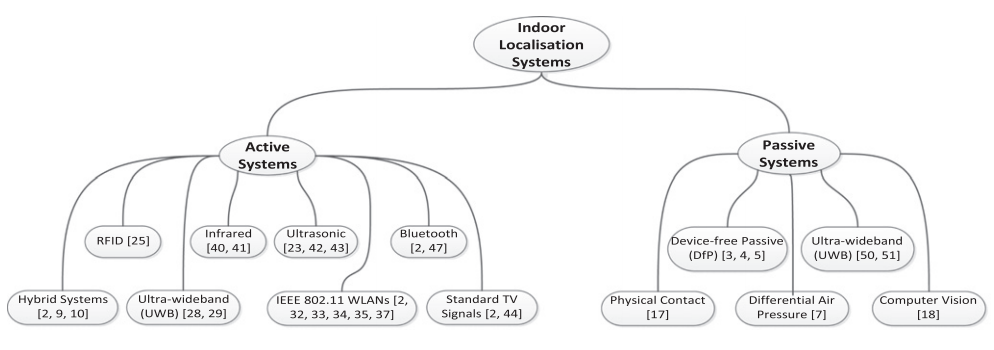
\includegraphics[scale=0.9]{pictures/indoor_loc}
	\caption{Unterkategorien von Indoor-Lokalisierung (Deak G.,  Curran K. \& Condell J., S. 2)}
\end{figure}

Im weiteren Verlauf wird jedes \textit{passive System} näher untersucht. Es wird die Funktionsweise sowie die Vor- und Nachteile des jeweiligen Systems erläutert.


\section{Sensorlose Indoor-Lokalisierung}
\subsection{Radio Frequency Identification}
Unter \textit{Radio Frequence Identification} (\textbf{RFID}) versteht man eine kontaktlose Identifikation mittels Funkübertragung. Oftmals kann man hierfür bereits vorhandene Wi-Fi-Netzwerke verwenden.\footnote{Vgl. Kivimäki T., Vuorela T., Peltola P. \& Vanhala J., S.  16} \\
Ein solches DfL-System (\textbf{Device-free Localization}) nutzt die Tatsache aus, dass die Präsenz eines menschlichen Körpers die Radiosignale beeinflussen.\footnote{Vgl. ebd.} Die verwendete Frequenz der Knotenpunkte liegt hierbei bei $2.4$Ghz, weil dies die Resonanzfrequenz von Wasser ist und der Mensch bekanntermaßen aus $70\%$ aus Wasser besteht.\footnote{Vgl. Deak G.,  Curran K. \& Condell J., S. 11}. Ein weiterer Pluspunkt ist auch, dass die Frequenz von $2.4$ Ghz bei \textit{IEEE Standards} wie $802.11b$ und $802.11g$ verwendet wird.\footnote{Vgl. Pirzada N.,Nayan Y., Subhan F., Hassan F., Khan M., S. 3}\\
Das \textit{DfP-System} auf Grundlage von \textit{RFID}, welches im Folgenden vorgestellt wird, misst die Änderungen von der erhaltenen \textit{Received Signal Strength Indication} (\textbf{RSSI}). Der Anwendungsbereich des vorgestellten Systems ist die Haussicherheit. Das System soll als Alarmanlage agieren und Eindringlinge lokalisieren bzw. detektieren können.\footnote{Vgl. Mah M., S. 2} Ein solches System besteht aus zwei Komponenten, den \textit{Access Points} (\textbf{AP})\footnote{Zugriffsknoten} und den \textit{Monitoring Points} (\textbf{MP})\footnote(Z. Dt. Kontrollknoten). Einen guten Überblick bietet die folgende Abbildung:\\

\begin{figure}[H]
	\centering
	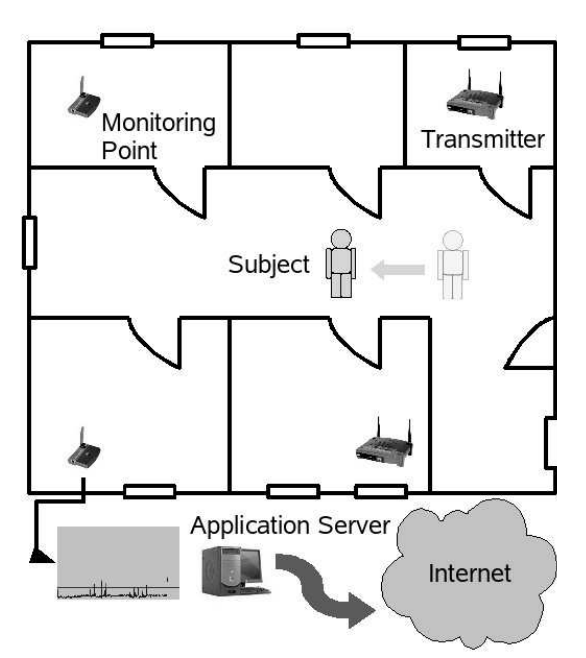
\includegraphics[width=0.5\textwidth]{pictures/rfid}
	\caption{RFID Indoor-Lokalisierung (Matthew Mah, S. 2)}
\end{figure}

In der obigen Abbildung erkennt man zwei \textbf{AP}, sowie einen \textbf{MP} und einen \textbf{DfP Server}, der die Berechnungen auf Grundlage der erhaltenen Signale durchführt. Als \textbf{MP} können dabei beliebige Computer verwendet werden.\footnote{Vgl. ebd.} Neben der eigentlichen Detektion (\textit{Monitoring Mode}) unterstützt das System noch zwei weitere Modi, welche nun näher beschrieben werden.\\

\begin{itemize}
\item \textbf{Monitoring Mode}: Dieser Modus nimmt jegliche Aktivität wahr, eignet sich somit für eine nächtliche Überwachung.
\item \textbf{Tracking mode}: Dieser Modus kann einen Eindringling orten und zusätzlich noch anhand der Daten der, die von den \textbf{MP} verzeichnet werden, verfolgen. Es kann nur ein Eindringling zu einem bestimmten Zeitpunkt geortet werden.
\item \textbf{DfP Mode}: Der \textit{DfP-Modus} kann mehrere Eindringlinge gleichzeitig orten und verfolgen.
\end{itemize}

Sobald ein Eindringling von einem \textbf{MP} detektiert wird, werden zusätzlich noch weitere \textit{Monitoring Points} kontaktiert und auf mögliche Detektionen überprüft. Erst danach kommt es zu einem Alarm des Gesamtsystems.\footnote{Vgl. ebd., S. 2 f.} Tests in kontrollierten Umgebungen ergaben zufriedenstellende Ergebnisse mit einer niedrigen Rate von \textit{False Positives}\footnote{Z. Dt. Falschpositiv} und einer hohen \textit{Detektionsrate}. Die beiden beiden folgenden Abbildungen zeigen dies nochmals graphisch auf.

\begin{figure}
\centering
\begin{minipage}{.5\textwidth}
  \centering
  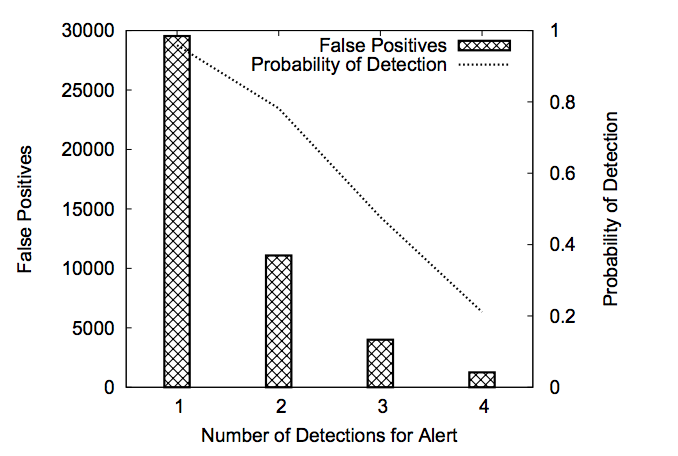
\includegraphics[scale=0.6]{pictures/false_pos}
  \caption*{False Positives}
\end{minipage}%
\begin{minipage}{.5\textwidth}
  \centering
  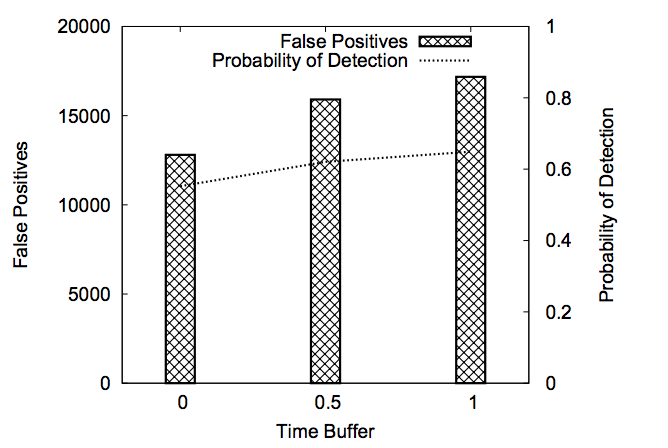
\includegraphics[scale=0.6]{pictures/detection}
  \caption*{Detection Rate}
\end{minipage}
\caption{Testergebnisse (Mah M., S. 9)}
\end{figure}

Dieses \textit{DfP-System} schnitt in den Tests zufriedenstellend ab, jedoch muss man auch auf mögliche Schwachstellen eingehen. Viele Parameter, die in den Algorithmen für die Detektion von Eindringlingen gebraucht werden haben direkten Einfluss auf die Sensibilität des Systems. Will man die Wahrscheinlichkeit eine Detektion zu verzeichnen erhöhen, wird gleichzeitig die Anzahl der \textit{False Positives} erhöht. Das Finden von Parametern, welche die Wahrscheinlichkeit von Detektionen erhöhen und gleichzeitig die Anzahl der \textit{False Positives} minimieren, ist ein Optimierungsproblem.\footnote{Vgl. ebd. S. 9}

\subsection{Ultra Wideband}

\subsection{Infrarot-Sensoren (besser an die Abbildung halten) vielleicht also Air Pressure}
\subsubsection{Bla}
\subsubsection{BlaBla}
\subsection{Drucksensoren}
\subsubsection{Bla}
\subsubsection{BlaBla}
\subsection{Computer-Vision}
\subsubsection{Bla}
\subsubsection{BlaBla}

\subsection{Fazit}

\subsection{Ausblick}

\newpage

\section{Quellenverzeichnis}
\subsection*{Literaturquellen}
\begin{itemize}[leftmargin=*]
\item[] \textbf{Sample}
\end{itemize}
\subsection*{Sonstige Quellen}
\begin{itemize}[leftmargin=*]
\item[] \textbf{Ehrlich, I.}: Indoor Localization, Online unter URL: \url{http://ifgi.uni-muenster.de/~muellerj/lbs06/proceedings/3-IndoorLocalization.pdf}
\item[] \textbf{Deak G., Curran K. \& Condell J.} A survey of active and passive indoor localisation systems, Online unter URL : \url{http://scisweb.ulster.ac.uk/~kevin/comcomsurvey.pdf}
\item[] \textbf{Kivimäki T., Vuorela T., Peltola P. \& Vanhala J.}: Indoor Localization, Online unter URL: \url{http://www.sersc.org/journals/IJSH/vol8_no1_2014/9.pdf}
\item[] \textbf{Pirzada N.,Nayan Y., Subhan F., Hassan F., Khan M.}: Device-Free Localization Technique for Indoor Detection and Tracking of Human Body, Online unter URL: \url{http://ac.els-cdn.com/S187704281402878X/1-s2.0-S187704281402878X-main.pdf?_tid=7bc6ad0e-12a4-11e5-95f4-00000aab0f02&acdnat=1434293516_4a2274a0ebfb932cf57c3f4f652c668f}
\item[] \textbf{M. Mah}: Device-Free Passive Localization (2007), Online unter URL: \url{https://www.cs.umd.edu/sites/default/files/scholarly_papers/MatthewMah_1.pdf}
\end{itemize}
\end{figure}